\begin{enumerate}[label=\thechapter.\arabic*,ref=\thechapter.\theenumi]
\item A speech signal, band limited to 4 kHz, is sampled at 1.25 times the Nyquist rate. The speech samples, assumed to be statistically independent and uniformly distributed in the range -5 V to +5 V, are subsequently quantized in an 8-bit uniform quantizer and then over a voice-grade AWGN telephone channel. If the ratio of transmitted signal power to channel noise power is 26 dB, the minimum channel bandwidth required to ensure reliable transmission of the signal with arbitrarily small probability of transmission error (\textit{rounded off to one decimal place}) is \rule{1cm}{0.15mm} kHz.
\hfill (GATE EC 2021)
\solution
\iffalse
\let\negmedspace\undefined
\let\negthickspace\undefined
\documentclass[journal,12pt,twocolumn]{IEEEtran}
\usepackage{cite}
\usepackage{amsmath,amssymb,amsfonts,amsthm}
\usepackage{algorithmic}
\usepackage{graphicx}
\usepackage{textcomp}
\usepackage{xcolor}
\usepackage{txfonts}
\usepackage{listings}
\usepackage{enumitem}
\usepackage{mathtools}
\usepackage{gensymb}
\usepackage{comment}
\usepackage[breaklinks=true]{hyperref}
\usepackage{tkz-euclide}
\usepackage{listings}
\usepackage{gvv}
\def\inputGnumericTable{}
\usepackage[latin1]{inputenc}
\usepackage{color}
\usepackage{array}
\usepackage{longtable}
\usepackage{calc}
\usepackage{multirow}
\usepackage{hhline}
\usepackage{ifthen}
\usepackage{lscape}

\newtheorem{theorem}{Theorem}[section]
\newtheorem{problem}{Problem}
\newtheorem{proposition}{Proposition}[section]
\newtheorem{lemma}{Lemma}[section]
\newtheorem{corollary}[theorem]{Corollary}
\newtheorem{example}{Example}[section]
\newtheorem{definition}[problem]{Definition}
\newcommand{\BEQA}{\begin{eqnarray}}
\newcommand{\EEQA}{\end{eqnarray}}
\newcommand{\define}{\stackrel{\triangle}{=}}
\theoremstyle{remark}
\newtheorem{rem}{Remark}
\begin{document}

\bibliographystyle{IEEEtran}
\vspace{3cm}

\title{GATE 2021 EC 23}
\author{EE23BTECH11007 - Aneesh Kadiyala$^{*}$% <-this % stops a space
}
\maketitle
\newpage
\bigskip

\renewcommand{\thefigure}{\theenumi}
\renewcommand{\thetable}{\theenumi}

\vspace{3cm}
\textbf{Question:} A speech signal, band limited to 4 kHz, is sampled at 1.25 times the Nyquist rate. The speech samples, assumed to be statistically independent and uniformly distributed in the range -5 V to +5 V, are subsequently quantized in an 8-bit uniform quantizer and then over a voice-grade AWGN telephone channel. If the ratio of transmitted signal power to channel noise power is 26 dB, the minimum channel bandwidth required to ensure reliable transmission of the signal with arbitrarily small probability of transmission error (\textit{rounded off to one decimal place}) is \rule{1cm}{0.15mm} kHz.
\hfill(GATE 2021 EC)
\\
\solution
\\
\fi
\begin{table}[h!]
    \centering
    \begin{tabular}{ | c | c | c | }
    \hline
    Parameter & Value & Description \\
    \hline
    $B_0$ & 4 kHz & Bandwidth of signal \\
    \hline
    $R_N$ & $2B_0$ & Nyquist Rate \\
    \hline
    $f_s$ & $1.25R_N$ & Sampling Frequency \\
    \hline
    $R$ & $nf_s$ & Data Rate \\
    \hline
    $C$ & $B\log_2{\brak{1 + \frac{P}{N}}}$ & Capacity of AWGN \\
    & & Channel with bandwidth $B$ \\
    \hline
    $10\log_{10}{\frac{P}{N}}$ & 26 dB & Signal to Noise Ratio \\
    \hline
\end{tabular}
    \caption{Input Parameters}
    \label{tab:2021ec23_1}
\end{table}

The signal is band limited to 4 kHz.
\begin{align}
B_0 &= 4\text{kHz} \\
%R_N &= 2B_0 \\
\implies R_N &= 8\text{kHz} \\
%f_s &= 1.25R_N \\
\implies f_s &= 10\text{kHz} \\
%R &= nf_s \\
R &= \brak{8}\brak{10\text{kHz}} \\
\implies R &= \brak{8}\brak{10^4}\text{ bits/second}
\end{align}
Channel capacity for an Additive White Gaussian Noise channel is
\begin{align}
C = B\log_2{\brak{1 + \frac{P}{N}}}\text{ bits/second}
\end{align}
where $P$ is the maximum channel power and $N$ is the noise power and $B$ is the channel bandwidth.
\begin{align}
10\log_{10}{\frac{P}{N}} &= 26\text{dB} \\
\implies \frac{P}{N} &= 10^{2.6} \\
&\approx 398.107
\end{align}
For reliable transmission:
\begin{align}
R &\le C \\
8\brak{10^4} &\le B\log_2{399.107} \\
B &\ge \frac{8\brak{10^4}}{\log_2{399.107}} \\
\implies B &\ge 9258.58\text{Hz}
\end{align}
$\therefore$ the minimum channel bandwidth required to ensure reliable transmission of the signal is $\approx9.26$ kHz.
\pagebreak

Consider a carrier signal which is amplitude modulated by a single-tone sinusoidal message signal with a modulation index of $50\%$. If the carrier and one of the sidebands are suppressed in the modulated signal, the percentage of power saved (rounded off to one decimal place) is \ldots.

\hfill(GATE EC 2021)
\solution
\iffalse
\let\negmedspace\undefined
\let\negthickspace\undefined
\documentclass[journal,12pt,twocolumn]{IEEEtran}
\usepackage{cite}
\usepackage{amsmath,amssymb,amsfonts,amsthm}
\usepackage{algorithmic}
\usepackage{graphicx}
\usepackage{textcomp}
\usepackage{xcolor}
\usepackage{txfonts}
\usepackage{listings}
\usepackage{enumitem}
\usepackage{mathtools}
\usepackage{gensymb}
\usepackage{comment}
\usepackage[breaklinks=true]{hyperref}
\usepackage{tkz-euclide} 
\usepackage{listings}
\usepackage{gvv}                                        
\def\inputGnumericTable{}                                 
\usepackage[latin1]{inputenc}                                
\usepackage{color}                                            
\usepackage{array}                                            
\usepackage{longtable}                                       
\usepackage{calc}                                             
\usepackage{multirow}                                         
\usepackage{hhline}                                           
\usepackage{ifthen}                                           
\usepackage{lscape}
\newtheorem{theorem}{Theorem}[section]
\newtheorem{problem}{Problem}
\newtheorem{proposition}{Proposition}[section]
\newtheorem{lemma}{Lemma}[section]
\newtheorem{corollary}[theorem]{Corollary}
\newtheorem{example}{Example}[section]
\newtheorem{definition}[problem]{Definition}
\newcommand{\BEQA}{\begin{eqnarray}}
\newcommand{\EEQA}{\end{eqnarray}}
\newcommand{\define}{\stackrel{\triangle}{=}}
\theoremstyle{remark}
\newtheorem{rem}{Remark}
\begin{document}

\bibliographystyle{IEEEtran}
\vspace{3cm}

\title{DISCRETE}
\author{EE23BTECH11006 - Ameen Aazam$^{*}$% <-this % stops a space
}
\maketitle
\newpage
\bigskip

\renewcommand{\thefigure}{\theenumi}
\renewcommand{\thetable}{\theenumi}

\vspace{3cm}
\textbf{Question :}
Consider a carrier signal which is amplitude modulated by a single-tone sinusoidal message signal with a modulation index of $50\%$. If the carrier and one of the sidebands are suppressed in the modulated signal, the percentage of power saved (rounded off to one decimal place) is \ldots.

\hfill(GATE EC 2021)

\solution
\fi
\begin{table}[htbp]
    \centering
    \begin{tabular}{|c|c|c|} \hline
      \textbf{Parameters} & \textbf{Values} & \textbf{Description} \\ \hline
      $m$ & $50\%$ & Percentage modulation \\ \hline
      $x_c\brak{t}$ & & Carrier signal \\ \hline
      $f_c\brak{t}$ & $1000 Hz$ & Carrier signal frequency \\ \hline
      $x_m\brak{t}$ & & Message signal \\ \hline
      $f_m\brak{t}$ & $25 Hz$ & Message signal frequency \\ \hline
      $A_c$ & & Amplitude of Carrier signal \\ \hline
      $P_t$ & & Total power of the modulated AP \\ \hline
      $P_c$ & $\frac{A_c^2}{2}$ & Power of the carrier signal \\ \hline
      $P_s$ & & Saved power \\ \hline
    \end{tabular}
    \vspace{3pt}
    \caption{Parameters}
\end{table}

The percentage modulation,
\begin{align}
    m=50\%=0.5
\end{align}
Suppose, we have the carrier signal as,
\begin{align}
    x_c\brak{t}=A_c\sin{\brak{2\pi f_ct}}
\end{align}
So the message signal,
\begin{align}
    x_m\brak{t}=mA_c\sin{\brak{2\pi f_mt}}
\end{align}
And the modulated signal,
\begin{align}
    y\brak{t}=A_c\brak{1+m\sin{\brak{2\pi f_mt}}}\sin{\brak{2\pi f_ct}}
\end{align}
Now the modulated signal in the frequency domain looks like,
\begin{figure}[h!]
    \centering
    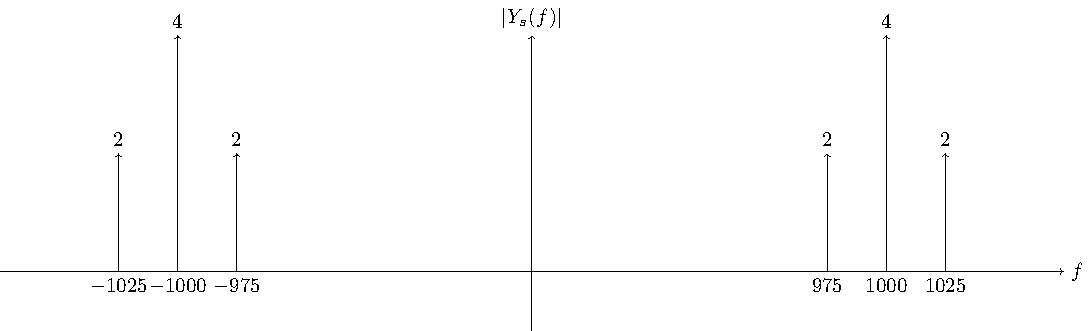
\includegraphics[width=\columnwidth]{2021/EC/22/figs/modulated.pdf}
    \caption{Modulated Signal}
\end{figure}
After the carrier signal and one of the side bands are removed,
\begin{figure}[h!]
    \centering
    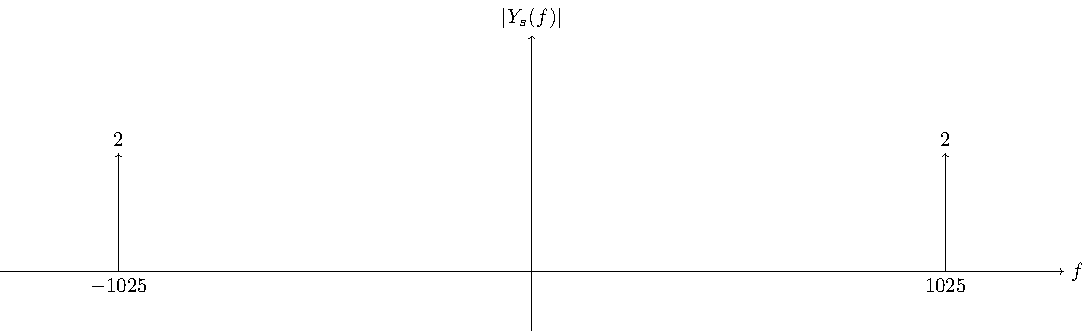
\includegraphics[width=\columnwidth]{2021/EC/22/figs/suppressed.pdf}
    \caption{Suppressed Signal}
\end{figure}
The total power is due to the carrier and the two sidebands,
\begin{align}
    P_t=P_c\sbrak{1+\frac{m^2}{2}}
\end{align}
Now as the carrier signal and one of the sidebands are suppressed then total saved power,
\begin{align}
    P_s=P_c\sbrak{1+\frac{m^2}{4}}
\end{align}
So percentage power saved,
\begin{align}
    &=\frac{P_s}{P_t}\times100\% \\
    &=\frac{P_c\sbrak{1+\frac{m^2}{4}}}{P_c\sbrak{1+\frac{m^2}{2}}}\times100\% \\
    &=\frac{1+\frac{1}{16}}{1+\frac{1}{8}}\times100\% \\
    &=94.44\%
\end{align}
Hence, the percentage power saved is $94.4\%$.
%\end{document}

\pagebreak
\end{enumerate}
